\documentclass{article}
\usepackage{subfiles}
\usepackage{forest}
\usetikzlibrary{shadows,arrows.meta}
\usepackage{float}
\usepackage{colortbl}
%A4 page size = 210mm, 297mm / inset total = size-margin
\usepackage[a4paper, total={190mm, 277mm}]{geometry}
\usepackage{fontspec}
%\setmainfont{TimesNewRoman}

\title{}
\author{}
\begin{document}
\large
  \subsection{Determine the MARR for this project with substrantiation}
  \begin{itemize}
    \item \textbf{Weighted Average Cost of Capital (WACC)}
      \begin{itemize}
        \item Cost of Debt: $K_{d_{(after \ tax)}}=Interest \ Rate \times (1-Tax \ Rate)$ 
        \item Cost of Equity: $Ke=R_f + \beta (R_m-R_f)$ 
        \item $WACC=(\frac{Equity}{(Total \ Capital)}K_e+\frac{Debt}{(Total \
          Capital)}K_{d_{after \ tax}})$ 

      \end{itemize}
    \item Project engages in a neice market, add \textbf{risk premium of 3\%}
    \item\textbf{Variables}
      \begin{itemize}
        \item $Tax \ Rate$ = 7\% \cite{sars}. 
        \item $Interest \ Rate$ = 9.75\% \cite{fatcat}
        \item (Risk free rate) $R_f$ = 7\% (ZA 10-year bond)
        \item (project risk prediction)$\beta$ =  1.2 (moderate risk)
        \item (Expected Market return) $R_m$ = 17\% \cite{simplywall} 
        \item Total Capital = R 1480236.28
        \item $Debt$ = R 1184189.03%(1480236.28*0.65)
        \item $Equity$ = R 296047.26 %(1480236.28*0.35)
        \item Debt fraction = $\frac{Debt}{Total \ Capital} = 0.8$
        \item Equity fraction = $\frac{Equity}{Total \ Capital} = 0.2$
      \end{itemize}
    \item\textbf{Opportuinity Cost from alternative industries}
      \begin{itemize}
        \item $Opportuinity \ Cost = RMPIC - RICP$
        \item In south africa stock market typically return 10-12\%
        \item Project return must exceed atleast 12\%
      \end{itemize}
    \item\textbf{Calculations}
      \begin{itemize}
        \item $K_{d_{(after \ tax)}}=9.75\%\times(1-7\%)=9.0675\%$
        \item $K_e=7\%+1.2(17\%-7\%)=19\%$
        \item $WACC=(Debt \ fraction \times K_{d_{(after \ tax)}}) + (Equity \
          fraction \times K_e)$ \\
          $WACC=(0.8*9.0675\%)+(0.2*19\%)$ \\
          $WACC=11.054\%$
        \item $MARR = max(WACC+Risk \ Premium,Opportuinity \ Cost) =
          max(11.054\%+3\%,12\%) = 14.054\%$ 
      \end{itemize}
      Project minimum rate of return 14.054\% beats opportuinity cost of 12\%
  \end{itemize}

  \subsection{NPV analysis}
  \textbf{Inputs: }
  \begin{itemize}
    \item Inital investment (Upfront cost) \\
      \begin{tabular}{|l|l|} \hline
        \textbf{Portfolio Initial Investment} & \textbf{Cost} \\ \hline
        Prodution Portfolio & R 1140902.95 \\ \hline
        Marketing Portfolio & R  123333.33 \\ \hline
        Logistics Portfolio & R  216000.00 \\ \hline
        Total &  R 1480236.28 \\ \hline
      \end{tabular}
    \item Discount rate (Inflation Rate) $r = 3.2\%$ \cite{inflate}
    \item Projected cash flow : obtained from Section 5: Cash flow tables.
    \item MARR 
  \end{itemize}
  \textbf{NPV calculaton:} \\
    \begin{itemize}
      \item $NPV = \sum_{t=0}^{n} \frac{CF_t}{(1 + r)^t}$
      \item $NPV = \sum_{t=0}^{n} PV_t$
    \end{itemize}
  \begin{figure}[H]
    \large
    \begin{tabular}{|l|l|l|l|} \hline 
      \multicolumn{4}{|c|}{\textbf{Mostlikely Revenue Projection}} \\ \hline
      \textbf{Year} & \textbf{Cash Flow (CF)} & \textbf{Discount Factor} (
      DF=$\frac{1}{(1+r)^t)}$) & \textbf{Present Value} ($DF \times CF$) \\
      \hline
      0 & R -1480236.28 & $\frac{1}{(1+0.032)^0}=1$ & R     -1480236.28 \\ \hline
      1 & R   601105.00 & $\frac{1}{(1+0.032)^1}=0.9689$ & R  582410.63 \\ \hline
      2 & R  1017115.25 & $\frac{1}{(1+0.032)^2}=0.9389$ & R  954969.51 \\ \hline
      3 & R  1294535.26 & $\frac{1}{(1+0.032)^3}=0.9098$ & R 1177768.18 \\ \hline
      \multicolumn{4}{|l|}{\textbf{$NPV =
      -1480236.28+582410.63+954969.51+1177768.18 = \textbf{R 1234912.04}$  
}} \\ \hline
    \end{tabular}
  \end{figure}
  \begin{figure}[H]
    \large
    \begin{tabular}{|l|l|l|l|} \hline 
      \multicolumn{4}{|c|}{\textbf{Worst case Revenue Projection}} \\ \hline
      \textbf{Year} & \textbf{Cash Flow (CF)} & \textbf{Discount Factor} (
      DF=$\frac{1}{(1+r)^t)}$) & \textbf{Present Value} ($DF \times CF$) \\
      \hline
      0 & R -1480236.28 & $\frac{1}{(1+0.032)^0}=1$ & R     -1480236.28 \\ \hline
      1 & R  -130468.75 & $\frac{1}{(1+0.032)^1}=0.9689$ & R -126411.17 \\ \hline
      2 & R   215306.53 & $\frac{1}{(1+0.032)^2}=0.9389$ & R  202151.30 \\ \hline
      3 & R   378151.44 & $\frac{1}{(1+0.032)^3}=0.9098$ & R  344042.18 \\ \hline
      \multicolumn{4}{|l|}{\textbf{$NPV =
      -1480236.28+-126411.17+202151.30+344042.18 = \textbf{R -1060453.97}$  
}} \\ \hline
    \end{tabular}
  \end{figure}
  \textbf{Analysis:}\\
  Project is worth presuing if most-likeley or slightly worse assumptions can be
  ensures else if the worst case scenario plays the project needs to be
  considered over a longer period of time (since upward tend is shown), else the
  project is not worth persuing.\\ \\ \\ 
  \textbf{Project Return Rate:}\\
  Calculate IRR in Excel: \\
  \begin{figure}[H]
    \centering
      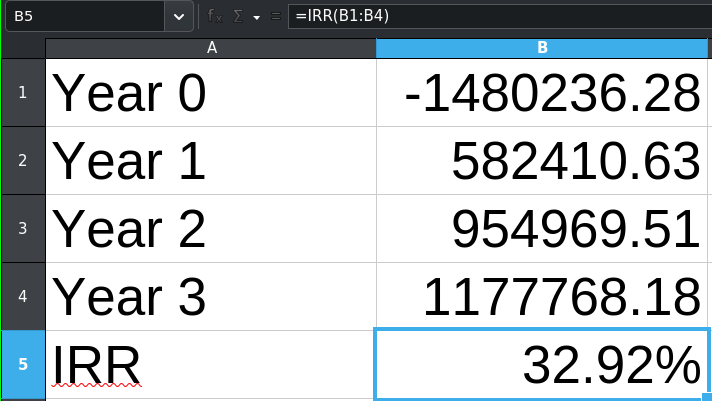
\includegraphics[width=0.7\linewidth]{figures/Excel_IRR.png}
    \caption{Excel calculation of IRR}
  \end{figure}
  IRR = 32.92\% which is much heigher that the MARR of 14.054\% \\
  It can be concluded that this is a worthy project to persue.

\end{document}
